\documentclass[10pt]{article}
\usepackage[utf8]{inputenc}
\usepackage[includehead, headheight=10mm, margin=15mm ]{geometry}
\usepackage{amsmath}
\usepackage{amsthm}
\usepackage{amsfonts}
\usepackage{xcolor}
\usepackage{graphicx}
\usepackage{titling}
\usepackage{fancyhdr}
\usepackage{listings}

\title{APPM 4600 Homework 7}
\author{Edward Wawrzynek}
\date{17 October 2024}

\newcommand*{\dif}{\mathop{}\!\mathrm{d}}
\renewcommand{\vec}{\mathbf}


\makeatletter
\def\@maketitle{%
  \newpage
  \null
  \vskip 1em%
  \begin{center}%
  \let \footnote \thanks
    {\LARGE \@title \par}%
    \vskip 1em%
    {\normalfont \@date}
  \end{center}%
  \par
  \vskip 1em}
\makeatother

\begin{document}

\pagestyle{fancy}
    \fancyhf{} % clear all header and footer fields
    \fancyhead[L]{\thetitle}
    \fancyhead[R]{\theauthor}

\makeatletter
\begin{center}
    {\Large \@title}
    \vskip 1mm
    {\normalfont \@date}
    \vskip 1em
\end{center}
\makeatother

\begin{enumerate}
  \item The code used to answer this question is listed at the end of the question. 
  
  \begin{enumerate}
    \item We have the polynomial \begin{align*}
      p_n(x) &= c_0 + c_1x + c_2x^2 + \dots + c_nx^n,
  \end{align*} which we wish to use to interpolate the data \(\{x_j, f(x_j)\}_{j=0}^n\). We plug these data points into the polynomial and have the system \begin{align*}
      \vec{y} = V\vec{c},
  \end{align*} where \(V\) is the matrix \begin{align*}
      V = \begin{bmatrix}
        1 & x_1 & x_1^2 & \dots & x_1^n \\
        1 & x_2 & x_2^2 & \dots & x_2^n \\
        & & \dots \\
        1 & x_n & x_n^2 & \dots & x_n^n 
      \end{bmatrix}.
  \end{align*} Thus, the coefficients \(\vec{c}\) are given by \begin{align*}
      \vec{c} = V^{-1}\vec{y}.
  \end{align*}

  \item We perform monomial interpolation on \begin{align*}
      f(x) = \frac{1}{1+(10x)^2}
  \end{align*} with an evenly spaced grid of interpolation points over \(x \in [-1, 1]\). Resulting polynomials are shown below for various number of points \(N\).

  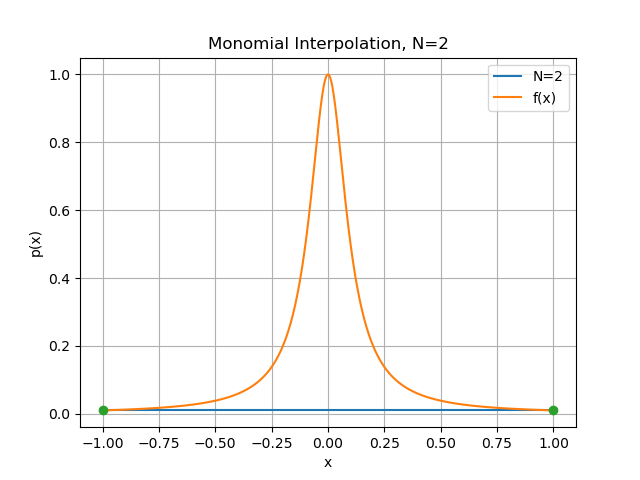
\includegraphics[width=0.49\textwidth]{mono2.png}
  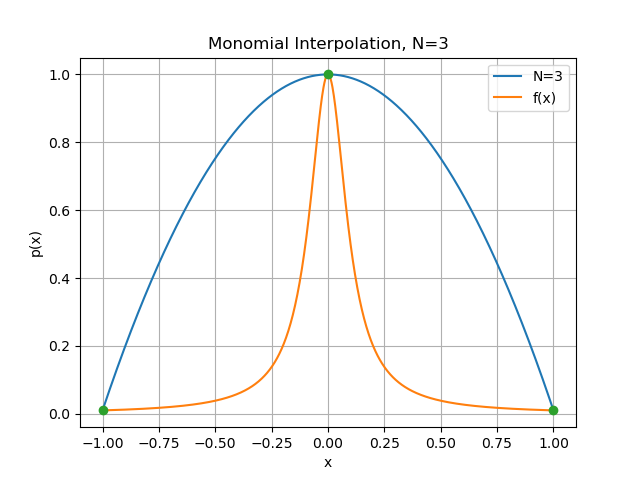
\includegraphics[width=0.49\textwidth]{mono3.png}
  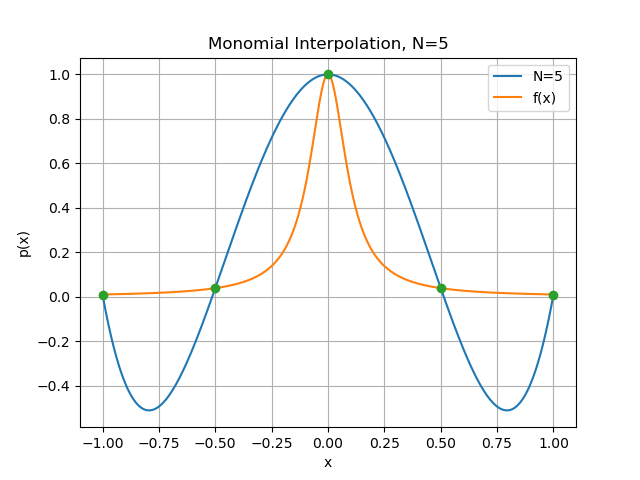
\includegraphics[width=0.49\textwidth]{mono5.png}
  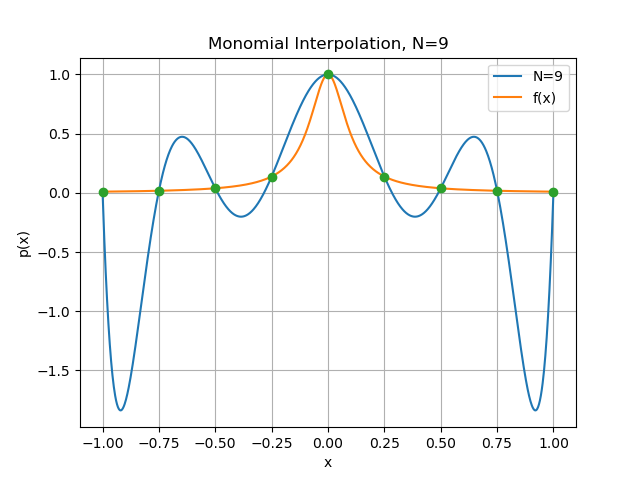
\includegraphics[width=0.49\textwidth]{mono9.png}
  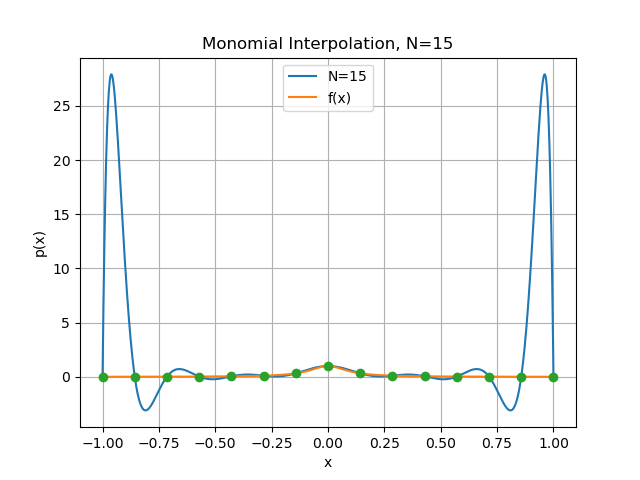
\includegraphics[width=0.49\textwidth]{mono15.png}
  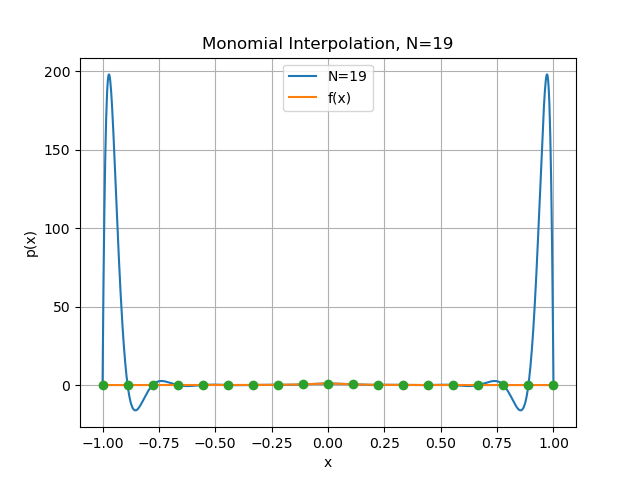
\includegraphics[width=0.49\textwidth]{mono19.png}

  With increasing \(N\), the polynomial is poorly behaved around the endpoints of the region, demonstrating the Runge phenomenon.

  {\small \lstinputlisting[language=Python]{hw7_1.py}}
  \newpage

  \end{enumerate}

  \item The code used in this question is listed at the end of the question. 
  
  We use the second Barycentric Lagrange formula, \begin{align*}
      p(x) = \frac{\sum_{j=0}^n \frac{w_j}{x-x_j}f(x_j)}{\sum_{j=0}^n \frac{w_j}{x-x_j}},
  \end{align*} where \begin{align*}
      w_j = \frac{1}{\prod_{i=0, i \neq j}^n (x_j-x_i)}.
  \end{align*}

  The interpolation shows the same Runge phenomenon as before, shown below.

  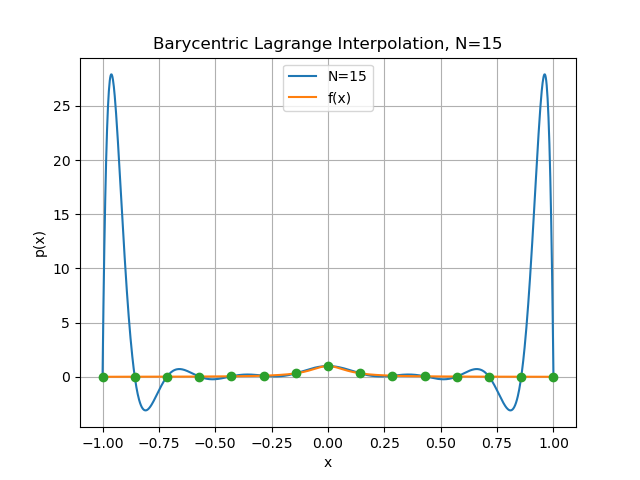
\includegraphics[width=0.49\textwidth]{bary15.png}
  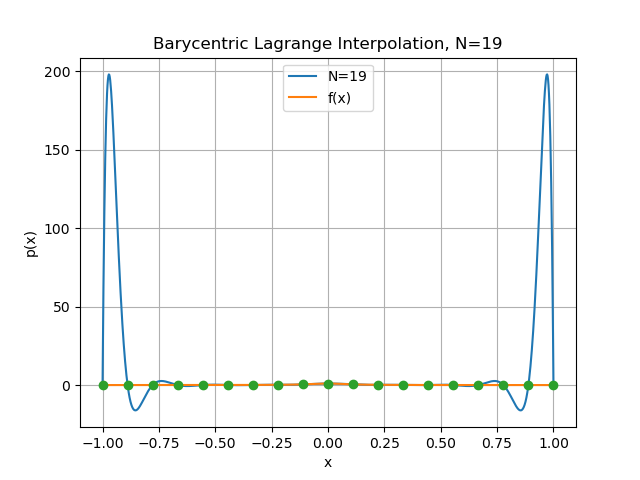
\includegraphics[width=0.49\textwidth]{bary19.png}

  However, the barycentric interpolation is much more stable than the monomial interpolation. For \(N=50\) interpolation points, both barycentric lagrange and monomial are plotted below. Barycentric Lagrange closely matches the interpolation points, whereas the monomial interpolation misses these points as a consequence of instability. 

  \begin{center}
  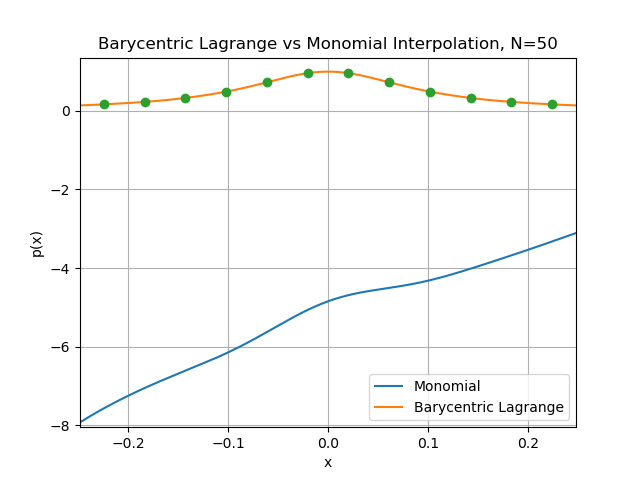
\includegraphics[width=0.5\textwidth]{hw7_2_1.png}
  \end{center}

  {\small \lstinputlisting[language=Python]{hw7_2.py}}

  \newpage

  \item The code used in this question is listed at the end of the question.
  
  We apply Barycnetric Lagrange interpolation over the function with Chebyshev points, \begin{align*}
      x_j = \cos \frac{(2j-1)\pi}{2N},\;i=1,\dots , N.
  \end{align*}

  The interpolation is shown below for various numbers of points \(N\). Notice that the polynomial remains bounded near the ends of the interval, even for large \(N\).

  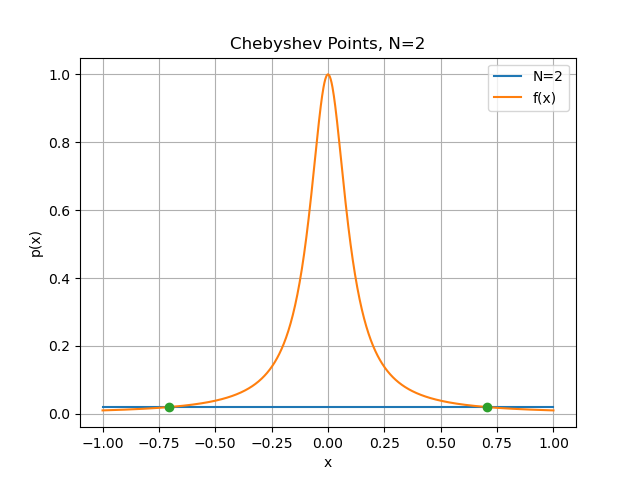
\includegraphics[width=0.49\textwidth]{cheb2.png}
  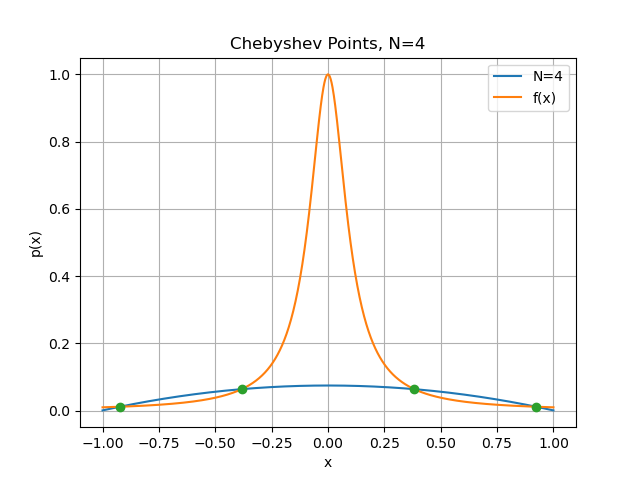
\includegraphics[width=0.49\textwidth]{cheb4.png}
  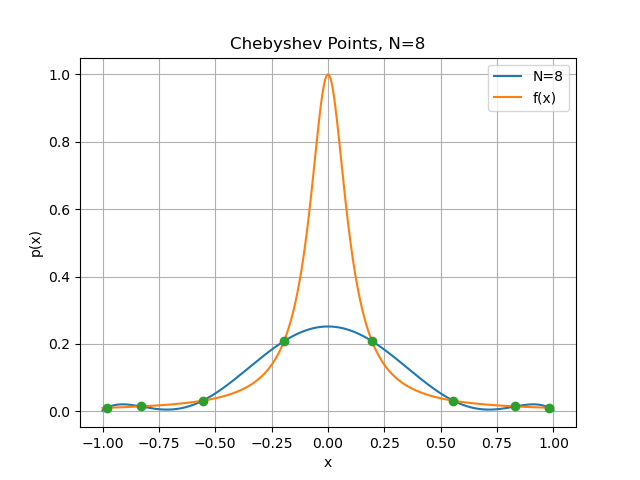
\includegraphics[width=0.49\textwidth]{cheb8.png}
  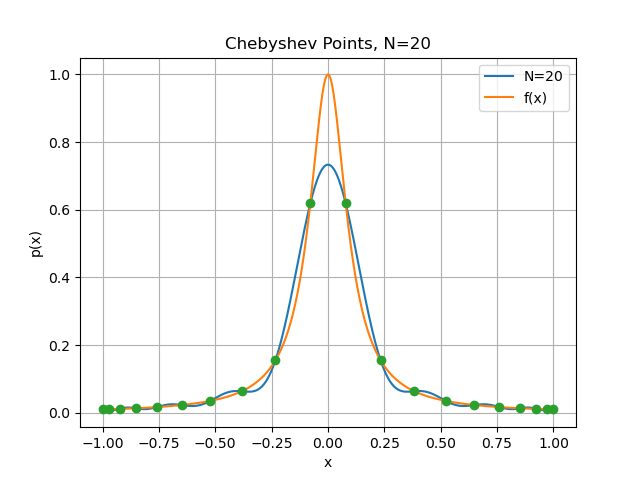
\includegraphics[width=0.49\textwidth]{cheb20.png}
  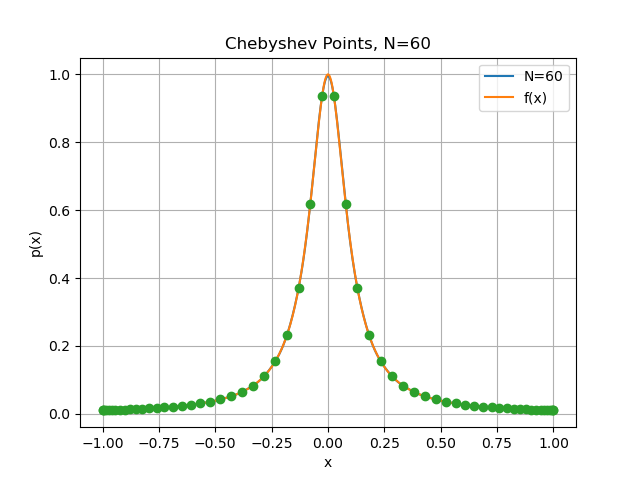
\includegraphics[width=0.49\textwidth]{cheb60.png}
  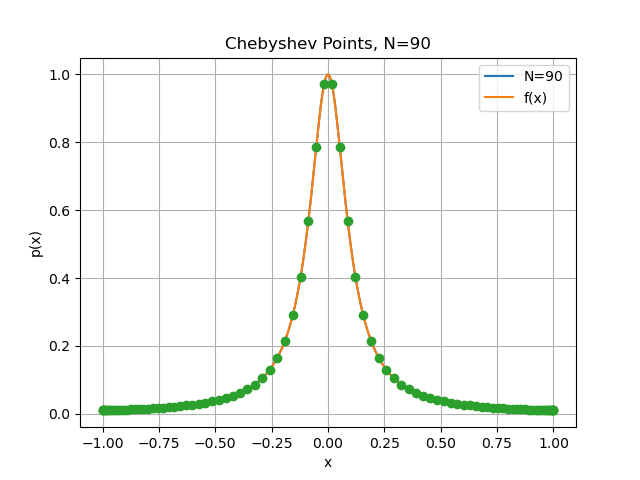
\includegraphics[width=0.49\textwidth]{cheb90.png}

  {\small \lstinputlisting[language=Python]{hw7_3.py}}

\end{enumerate}


\end{document}
